\documentclass{article}

\usepackage[dutch]{babel}
\usepackage[margin=3cm]{geometry}
\usepackage{graphicx}
\usepackage{float}
\usepackage{caption}
\usepackage{hyperref}
\usepackage{amsmath}
\usepackage{wrapfig}
\usepackage[parfill]{parskip}

% fonts
\usepackage[T1]{fontenc}
\usepackage{helvet}
\renewcommand{\familydefault}{\sfdefault}

\graphicspath{{img/}}
 
\newcommand{\bold}[1]{\textbf{#1}}

%Define the listing package
\usepackage{listings} %code highlighter
\usepackage{upquote}
\usepackage{color} %use color
\definecolor{mygreen}{rgb}{0,0.6,0}
\definecolor{mygray}{rgb}{0.5,0.5,0.5}
\definecolor{mymauve}{rgb}{0.58,0,0.82}

\begin{document}

\begin{titlepage}
    \author{Tuur Vanhoutte}
    \title{IoT Cloud}
\end{titlepage}

\pagenumbering{gobble}
\maketitle
\newpage
\tableofcontents
\newpage

\pagenumbering{arabic}

\section{Cloud computing}

= the practice of using a network of remote servers hosted on the Internet to store, manage, and process data, rather than a local server or a personal computer.

\subsection{Enkele eigenschappen}
\begin{itemize}
    \item Geen eigen hardware (we kopen niets aan)
    \item Ongelimiteerde computing power
    \item Ongelimiteerde storage capaciteit
    \item Scaling up and down op aanvraag of
    automatisch
    \item Scaling in en out op aanvraag of
    automatisch
    \item Geografische spreiding
    \item Pay what you use
\end{itemize}

\begin{figure}[H]
    \centering
    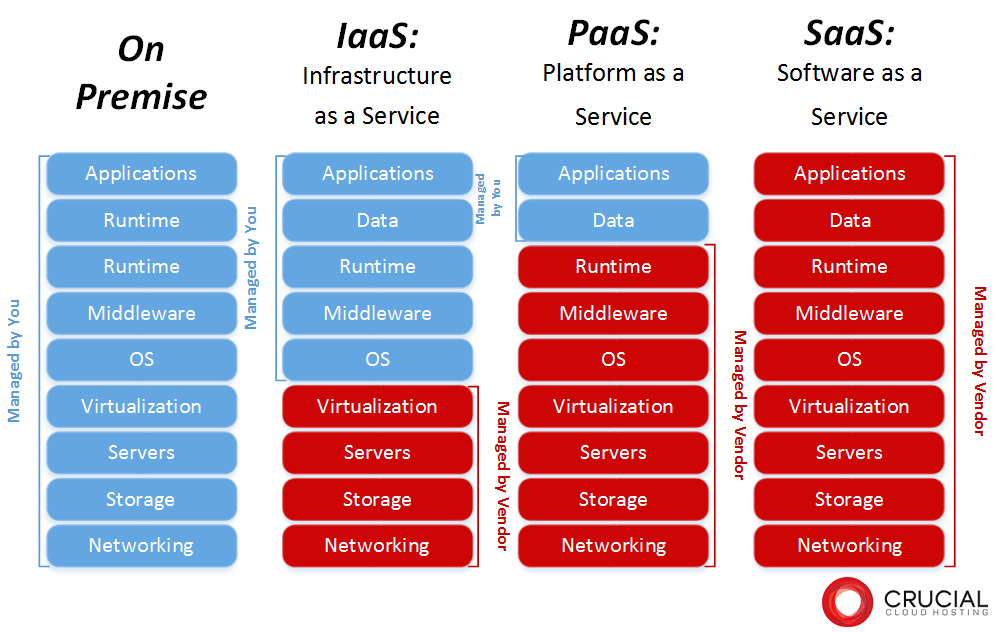
\includegraphics[width=0.7\textwidth]{cloud-hosting.png}
    \caption{}
\end{figure}


\subsection{On premise (eigen servers)}

\begin{itemize}
    \item IT Afdeling is verantwoordelijk voor ALLES
    \item Back-up \& recovery
    \item Aankoop hardware
    \item Scaling...
    \item Meeste vrijheid om te werken
    \item Soms investeren in hardware die je maar beperkt aantal dagen nodig hebt
    \item Vb: webshop en kerstperiode
    \item Soms verplicht door wetgeving
    \item Medische data
    \item Financial data
    \item Gebrek aan vertrouwen bij public cloud provider (cfr NSA)
\end{itemize}

\subsection{Hybrid Cloud (On Premise \& Cloud)}
Makes use of existing in-house infrastructure and Netplan cloud services to provide the best of both worlds.

\begin{itemize}
    \item Eigen datacenter koppelen aan cloud omgeving
    \item Bepaalde diensten draaien in cloud omgeving andere in eigen datacenter
    \item Zware load laten uitvoeren op de cloud
    \item Bepaalde data mag NIET in cloud opgeslagen worden vb: medical
    \item Kan ook gebruikt worden in back-up scenario’s
\end{itemize}

\subsection{IaaS: Infrastructure as a Service}

\begin{itemize}
    \item Geen eigen hardware kopen
    \item We huren virtual machines in Cloud omgeving
    \item Systeem beheerder moet zelf server configureren en beveiligen en updaten
    \item Veel flexibiliteit naar software installatie toe
    \item Zeer veel vrijheid maar ook verantwoordelijkheid
    \item Je moet zelf scaling doen (soms auto scaling mogelijk)
    \item Veel gebruik voor migratie bestaande On Premise naar cloud
\end{itemize}

\subsubsection{Voorbeelden}
\begin{itemize}
    \item Amazon Web Services (AWS)
    \item Microsoft Azure
    \item IBM Bluemix
    \item Google Cloud platform
\end{itemize}

\subsection{PaaS: Platform as a Service}

\begin{itemize}
    \item Geen systeembeheerder nodig
    \item Ontwikkelaar maakt applicatie en "plaatst" deze op Cloud platform
    \item We moeten ons geen zorgen maken in servers, hosting, back-ups, scaling,... het platform zal dit voor ons beheren
    \item Zeer veel flexibiliteit
\end{itemize}

We zullen vooral dit gebruiken in IoT Cloud module.

\subsubsection{Talen}
\begin{itemize}
    \item ASP.NET Core
    \item NodeJS
    \item Python
    \item Java
    \item PHP
\end{itemize}

\subsubsection{Voorbeelden}
\begin{itemize}
    \item Amazon Web Services (AWS)
    \item Microsoft Azure
    \item IBM Bluemix
    \item Google Cloud platform
    \item Heroku
\end{itemize}

\subsection{SaaS}
\begin{itemize}
    \item Software draait meestal niet lokaal (uitzondering Adobe \& Office)
    \item We betalen per maand/gebruiker
    \item Flexibele abonnementen, snel op te zetten
    \item We moeten geen rekening houden met back-ups en uptime
\end{itemize}

\subsubsection{Voorbeelden}
\begin{itemize}
    \item salesforce
    \item Office 365
    \item Dropbox, OneDrive, Google Drive, iCloud
    \item Gmail
    \item Adobe Creative Cloud
\end{itemize}

\subsection{Belangrijkste vendors}
\begin{itemize}
    \item Amazon Web Services
    \item Microsoft Azure
    \item Google Cloud Platform
\end{itemize}

\begin{figure}[H]
    \centering
    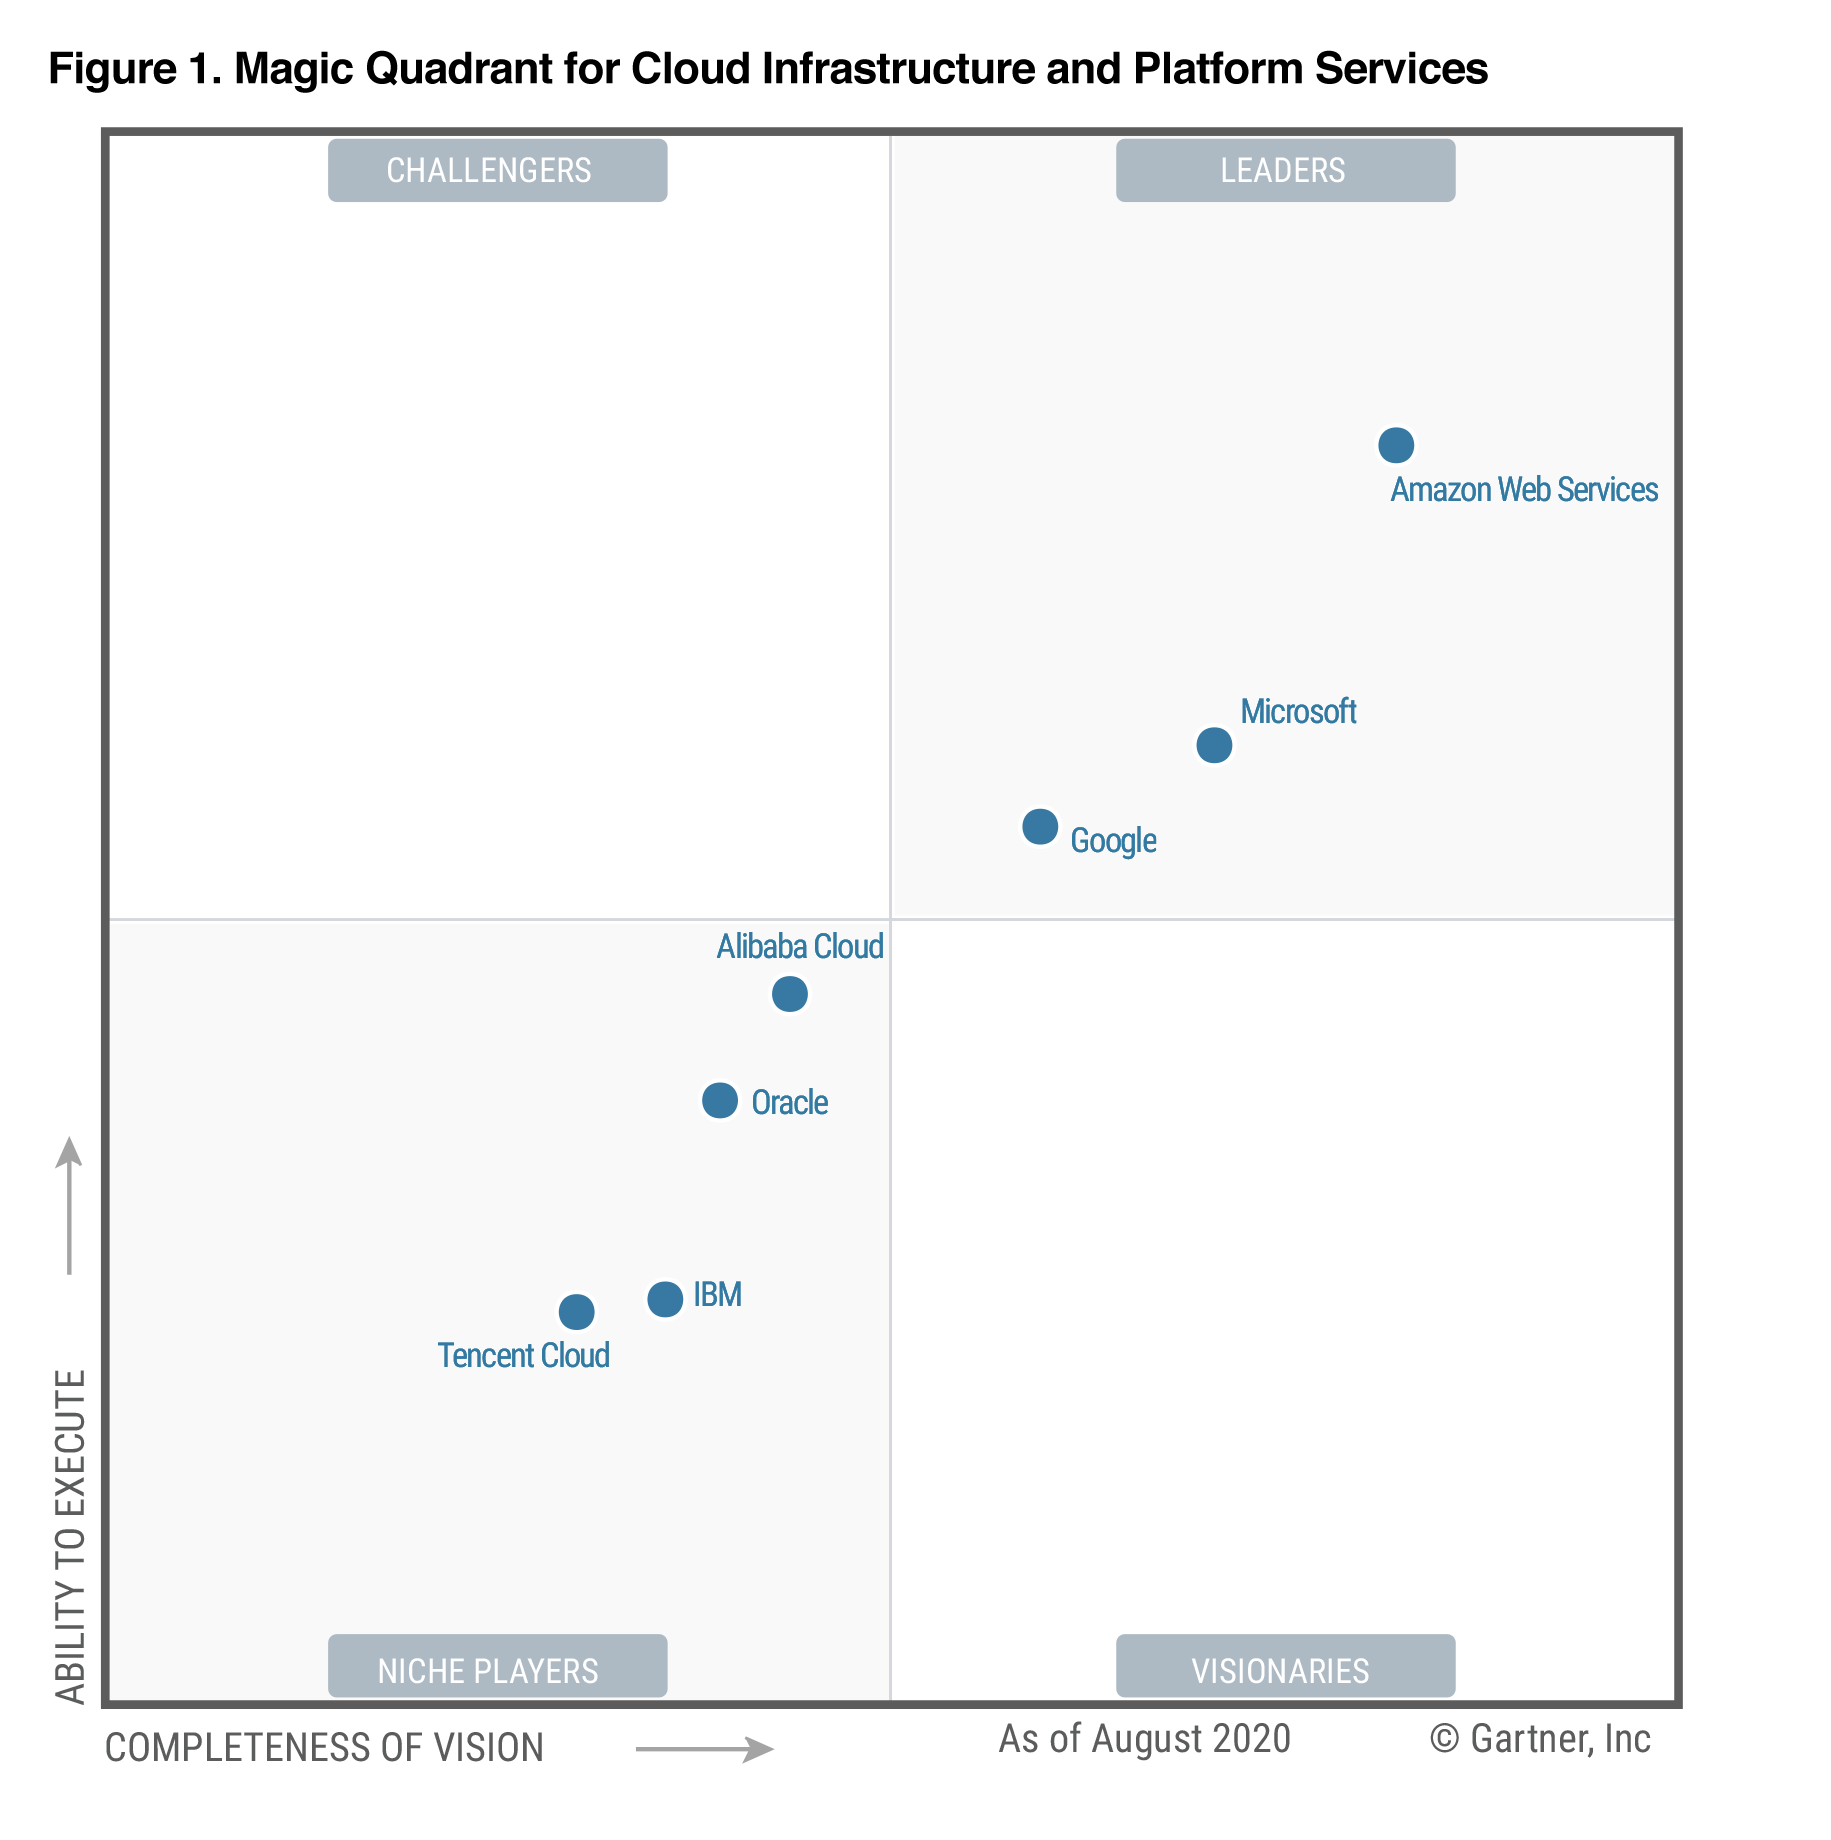
\includegraphics[width=0.5\textwidth]{magic-quadrant.png}
    \caption{}
\end{figure}



\section{Microsoft Azure}
We kiezen voor Microsoft Azure omwille van:
\begin{itemize}
    \item Zowel .NET als Open Source (PHP, Java, Node, Python, Flask, Docker...)
    \item Meeste opties en mogelijkheden
    \item Zeer lage instapdrempel voor studenten
\end{itemize}


\subsection{Azure Portal}

Inloggen via \url{portal.azure.com}

\begin{itemize}
    \item Beheren van uw Cloud services en applicaties
    \item Inloggen met Howest Account
    \item Kies een voldoende sterk passwoord en gebruik 2FA
\end{itemize}

\subsection{Azure subscription}
\begin{itemize}
    \item Abonnement
    \item Dit zal bepalen hoe ze factureren
    \item Verschillende opties:
    \begin{itemize}
        \item Credits op voorhand
        \item Pay by use
    \end{itemize}
    \item In de praktijk: per klant een subscription
    \item Voor de lessen: we hebben de "gratis subscription"
    \item Meerdere subscriptions mogelijk
\end{itemize}

\subsection{Resource Group}

\begin{figure}[H]
    \centering
    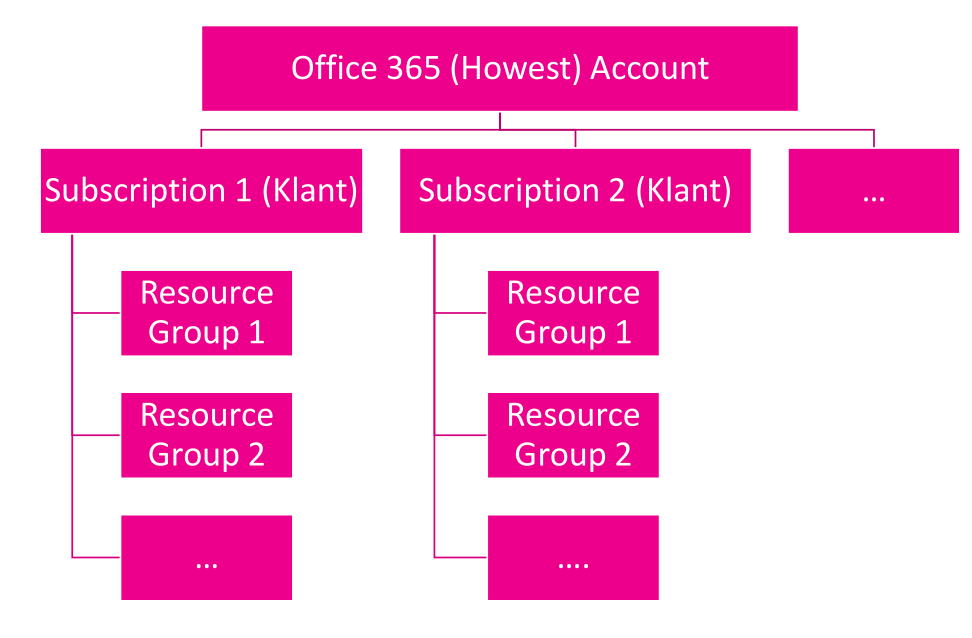
\includegraphics[width=0.5\textwidth]{resource-group.png}
    \caption{Resource groups}
\end{figure}

\begin{itemize}
    \item Logische container
    \item Per project
    \item Per soort services
    \begin{itemize}
        \item Storage
        \item Webservers
        \item Fileservers
        \item SQL, Blob, \dots
    \end{itemize}
    \item Je kiest dit zelf
    \item Makkelijk om te testen, je kan een volledige container verwijderen zonder dat je alles apart moet verwijderen
    \item Toegangsrechten per container zijn mogelijk
    \begin{itemize}
        \item via Office 365 account
    \end{itemize}
    \item Je kies datacenter locatie van je resource group, niet alle resources moeten op dezelfde locatie staan als je resource group.
\end{itemize}

\subsection{Azure Virtual Machines}
\begin{itemize}
    \item Eigen server op Azure omgeving
    \item Meestal on-premise (server op bedrijf) die we virtueel verplaatsen naar Azure
    \item Heel wat mogelijkheden
    \begin{itemize}
        \item File servers
        \item Database servers
        \item Webservers
        \item Application servers
        \item ...
    \end{itemize}
    \item Toegang tot resources op server die niet mogelijk zijn via een web applicatie
    \begin{itemize}
        \item Bv. communicatie met oude software pakketten
        \item Bv. Genereren van Word/Excel documenten
        \item \dots
    \end{itemize}
\end{itemize}

\subsubsection{Waarom?}
Wanneer je volledige controle wenst over je machine

\begin{itemize}
    \item Volledige controle == volledige verantwoordelijkheid!
    \begin{itemize}
        \item Niet te onderschatten
        \item Security, patching, scaling
    \end{itemize}
    \item Windows
    \item Linux
\end{itemize}

\subsubsection{Maintenance}

\begin{itemize}
    \item Planned maintenance
    \begin{itemize}
        \item Updates van het Azure platform (stabiliteit, security, performance)
        \item Soms moet de VM herstarten
    \end{itemize}
    \item Unplanned maintenance
    \begin{itemize}
        \item Storing in de onderliggende architectuur (netwerk-, disk-, rack-problemen)
        \item Azure zal automatisch VM verplaatsen naar werkende infrastructuur
    \end{itemize}
\end{itemize}

Hoe kan ik mijn VM `up and running' houden?
\begin{itemize}
    \item Availability set
    \begin{itemize}
        \item Garantie van 99.95\% uptime
        \item Minstens 2 virtual machines nodig
        \item Duurder
    \end{itemize}
\end{itemize}

\subsection{Azure Web App}
\begin{itemize}
    \item Azure Platform Service
    \item Laat ons toe om webapps online te plaatsen
    \item We moeten GEEN eigen server aanmaken
    \item We moeten GEEN webserver configureren
    \item Click \& go
    \item Ondersteuning voor:
    \begin{itemize}
        \item ASP.NET (Core)
        \item PHP
        \item Python Flask
        \item Java
        \item Node.JS
        \item \dots
    \end{itemize}
    \item Makkelijkste manier om uw applicatie online te krijgen, easy deployment
    \item Eenvoudige te koppelen aan een GitHub Repository
    \item Autoscale (not free)
    \item Monitoring
    \item Staging mode
\end{itemize}

\subsubsection{Free}
= gratis plan voor Azure Web App

\begin{itemize}
    \item Gedeelde server met andere web apps
    \item Je weet niet welke server, is transparant voor gebruiker
    \item 1GB storage
    \item Beperking op trafiek per dag: 165MB
\end{itemize}

\subsubsection{Shared}
\begin{itemize}
    \item Gedeelde server
    \item 1GB storage
    \item Mogelijkheid tot DNS vb: www.mijnnaam.be
\end{itemize}

\subsubsection{Basic, Premium}
\begin{itemize}
    \item App service plan $\Rightarrow$ eigen server, dus niks delen met derden (je kan niet inloggen op die server)
    \item SSL
    \item Custom domains
    \item CPU keuze
    \item Memory keuze
    \item Scaling tot 3 toestellen
\end{itemize}

\subsection{Scaling}

\subsubsection{Scale Up}
\begin{itemize}
    \item = vertical scaling
    \item Server krachtiger maken, meer memory en CPU
\end{itemize}

Pros: 
\begin{itemize}
    \item Minder energie dan scale out
    \item Eenvoudiger te implementeren
    \item Minder licenties (n.v.t. op Azure Web App)
\end{itemize}

Cons:

\begin{itemize}
    \item Duurder
    \item Indien we maar 1 machine gebruiken: $\Rightarrow$ hardware failure en toepassing is down
\end{itemize}


\subsubsection{Scale Out}
\begin{itemize}
    \item = horizontal scaling
    \item Meerdere machiens maar minder krachtig
\end{itemize}

Pros: 
\begin{itemize}
    \item Goedkoper
    \item Betere bescherming bij hardware failure, hebt meerdere machines
\end{itemize}

Cons:

\begin{itemize}
    \item Meer licenties nodig (n.v.t. op Azure)
    \item Meer plaats in datacenter
    \item Meer energieverbruik
    \item Complexer netwerk
    \item Soms toepassing aanpassen
\end{itemize}

\subsection{Azure SQL}

\begin{itemize}
    \item 
    \item SQL Server Database op Cloud platform
    \item We moeten zelf geen hardware/software aankopen
    \item Niet verantwoordelijk voor backups
    \item Eenvoudige schalen bij zware loads
    \item 3 opties
    \begin{itemize}
        \item Serverless Managed Database (onze voorkeur)
        \item SQL Managed Instance
        \item SQL Virtual Machine
    \end{itemize}
\end{itemize}

\subsubsection{SQL Server Cloud Based}
\begin{itemize}
    \item Compatible met SQL server 2012
    \item Te beheren via Enterprise manager
    \item Werkt zoals een gewone SQL server
    \item Connecteren is mogelijk via:
    \begin{itemize}
        \item .NET
        \item Python
        \item PHP
        \item Node
        \item \dots
    \end{itemize}
    \item High Availability
    \begin{itemize}
        \item Replicatie over 3 servers (default)
        \item Automatische Back-ups
    \end{itemize}
    \item Database draait op een server
    \item Verschillende pricing mogelijkheden
\end{itemize}

\subsubsection{Eigenschappen}
\begin{itemize}
    \item Database draait op een server
    \item Verschillende pricing mogelijkheden
\end{itemize}

\subsubsection{Security}
Azure FireWall: IP adres van je netwerk toelaten

\subsubsection{Azure DTU}
\begin{itemize}
    \item DTU = Database Transaction Units
    \item Soort `munteenheid'
    \item Gemengde eenheid van:
    \begin{itemize}
        \item CPU
        \item Memory
        \item I/O
    \end{itemize}
    \item Deze resources krijg je ter beschikking
    \item Hoe meer DTU, hoe meer power, hoe duurder
    \item \url{https://docs.microsoft.com/en-us/azure/sql-database/sql-database-what-is-a-dtu}
    \item vCores = virtuele CPUs die de service mag gebruiken
\end{itemize}

\subsubsection{Throttling}
= Onderbreken van database communicatie omdat je teveel resources (DTU's) gebruikt (zelf voor retry zorgen).

\begin{figure}[H]
    \centering
    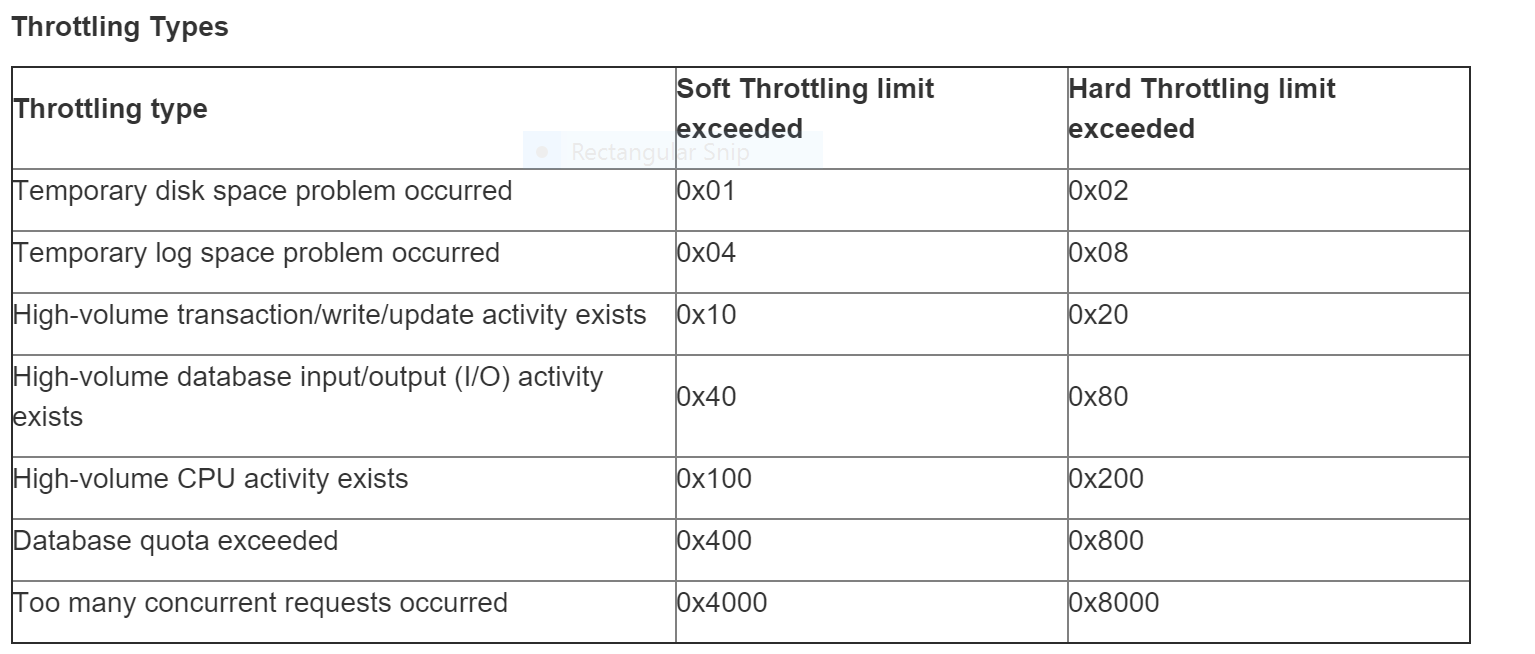
\includegraphics[width=0.8\textwidth]{azure-throttling.png}
    \caption{Throttling types}
\end{figure}

\begin{figure}[H]
    \centering
    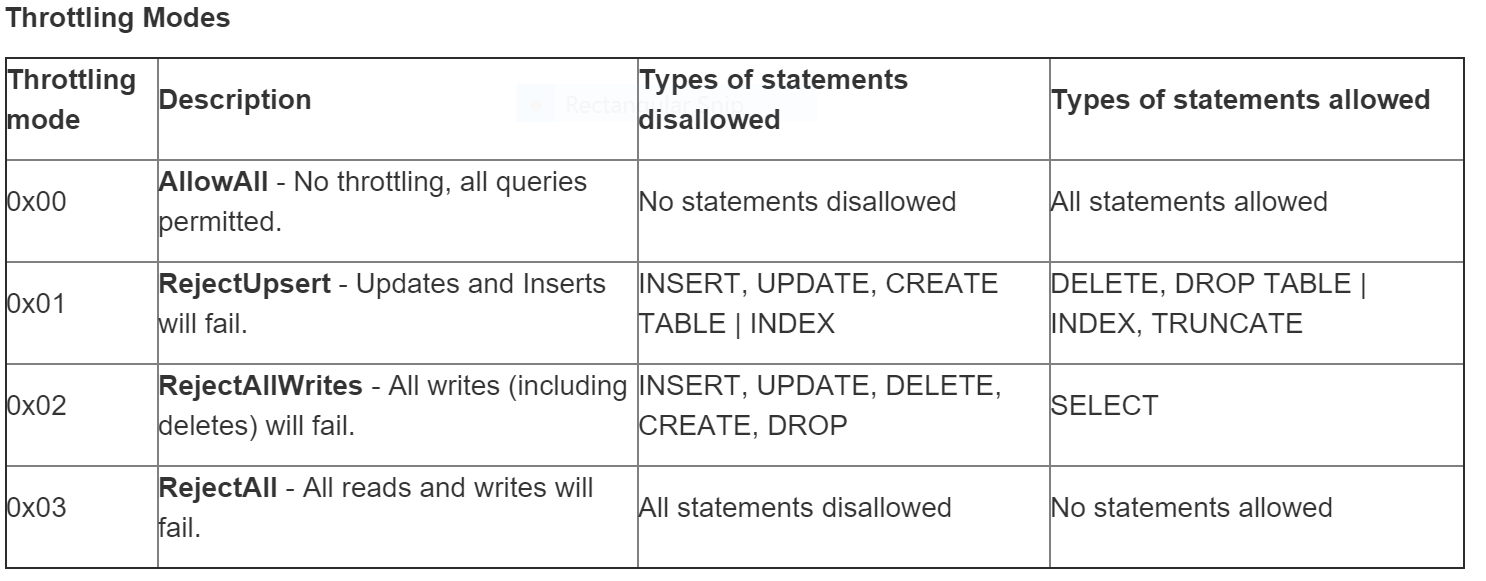
\includegraphics[width=0.8\textwidth]{azure-throttling-modes.png}
    \caption{Throttling modes}
\end{figure}

\begin{figure}[H]
    \centering
    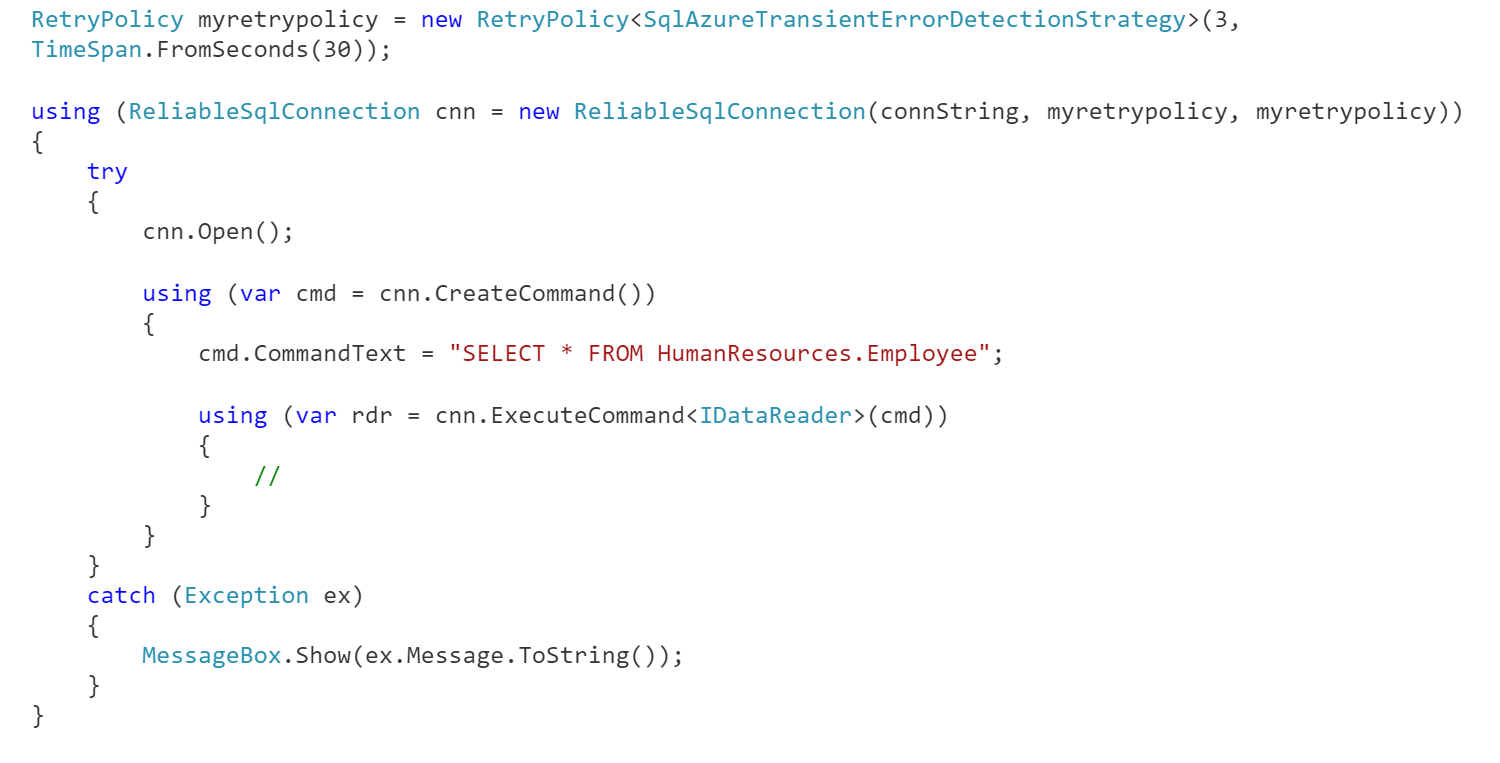
\includegraphics[width=0.8\textwidth]{azure-sql-command-ex.png}
    \caption{Voorbeeld SQL command in C\#}
\end{figure}


\subsubsection{Resources}
\begin{itemize}
    \item \url{https://msdn.microsoft.com/en-us/library/azure/dn338079.aspx}
    \item \url{http://geekswithblogs.net/ScottKlein/archive/2012/01/27/understanding-sql-azure-throttling-and-implementing-retry-logic.aspx}
\end{itemize}

\subsubsection{Azure Database for MySQL}

\begin{itemize}
    \item Toegang via MySQL Workbench
    \item Werkt zoals een gewone MySQL DB
    \item Je moet geen eigen servers opzetten, is volledig managed
    \item Automatische Back-ups
\end{itemize}

\subsection{Azure \& Internet of Things}

\subsubsection{Waarom is Azure belangrijk voor IoT?}

\begin{itemize}
    \item Azure Event Hubs
    \begin{itemize}
        \item Ontvangen van berichten afkomstig van toestellen
    \end{itemize}
    \item \textcolor{red}{Azure IoT Hub}
    \begin{itemize}
        \item Ontvangen van berichten
        \item Versturen van berichten naar toestellen
    \end{itemize}
    \item Azure Streaming Analytics
    \begin{itemize}
        \item Verwerken van events afkomstig van Event Hubs en IoT Hub
    \end{itemize}
\end{itemize}

\bold{Bovenstaande zeer belangrijk voor ons!}

\begin{figure}[H]
    \centering
    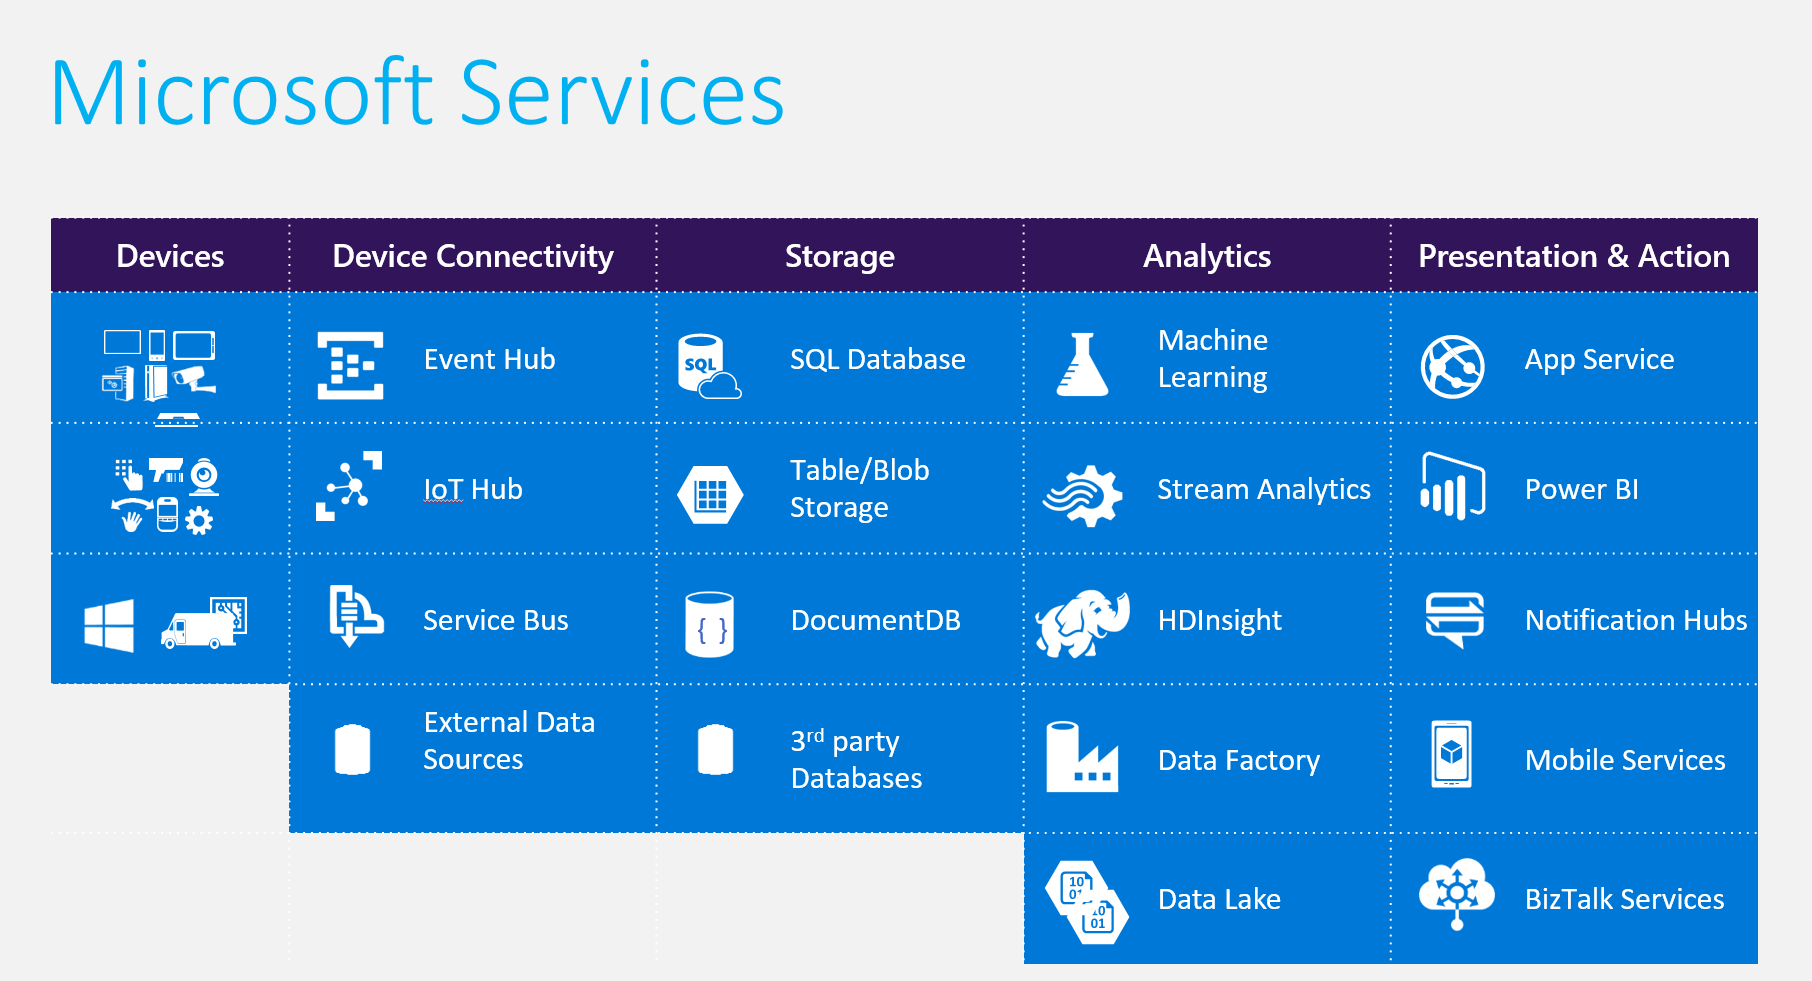
\includegraphics[width=0.8\textwidth]{azure-iot-microsoft-services.png}
    \caption{Microsoft Services}
\end{figure}

\subsection{Azure CLI}

\subsubsection{Azure Portal}

\begin{itemize}
    \item OK voor dagelijks gebruik
    \item Niet makkelijk te automatiseren
    \item Wat als ik 100 sites nodig heb?
    \item Wat als ik 50 servers nodig heb?
\end{itemize}

\subsubsection{Oplossing: Azure CLI 2.0}
\begin{itemize}
    \item Commandline Azure resources aanmaken
    \item Makkelijk met scripts
    \item Ideaal voor DevOps
\end{itemize}

\subsection{Bash/Powershell}

\begin{itemize}
    \item Bash commandline in portal
    \item Alles wat je via UI kan doen kan je ook via commandline in de portal
\end{itemize}

\subsection{Andere Azure onderdelen}
\begin{figure}[H]
    \centering
    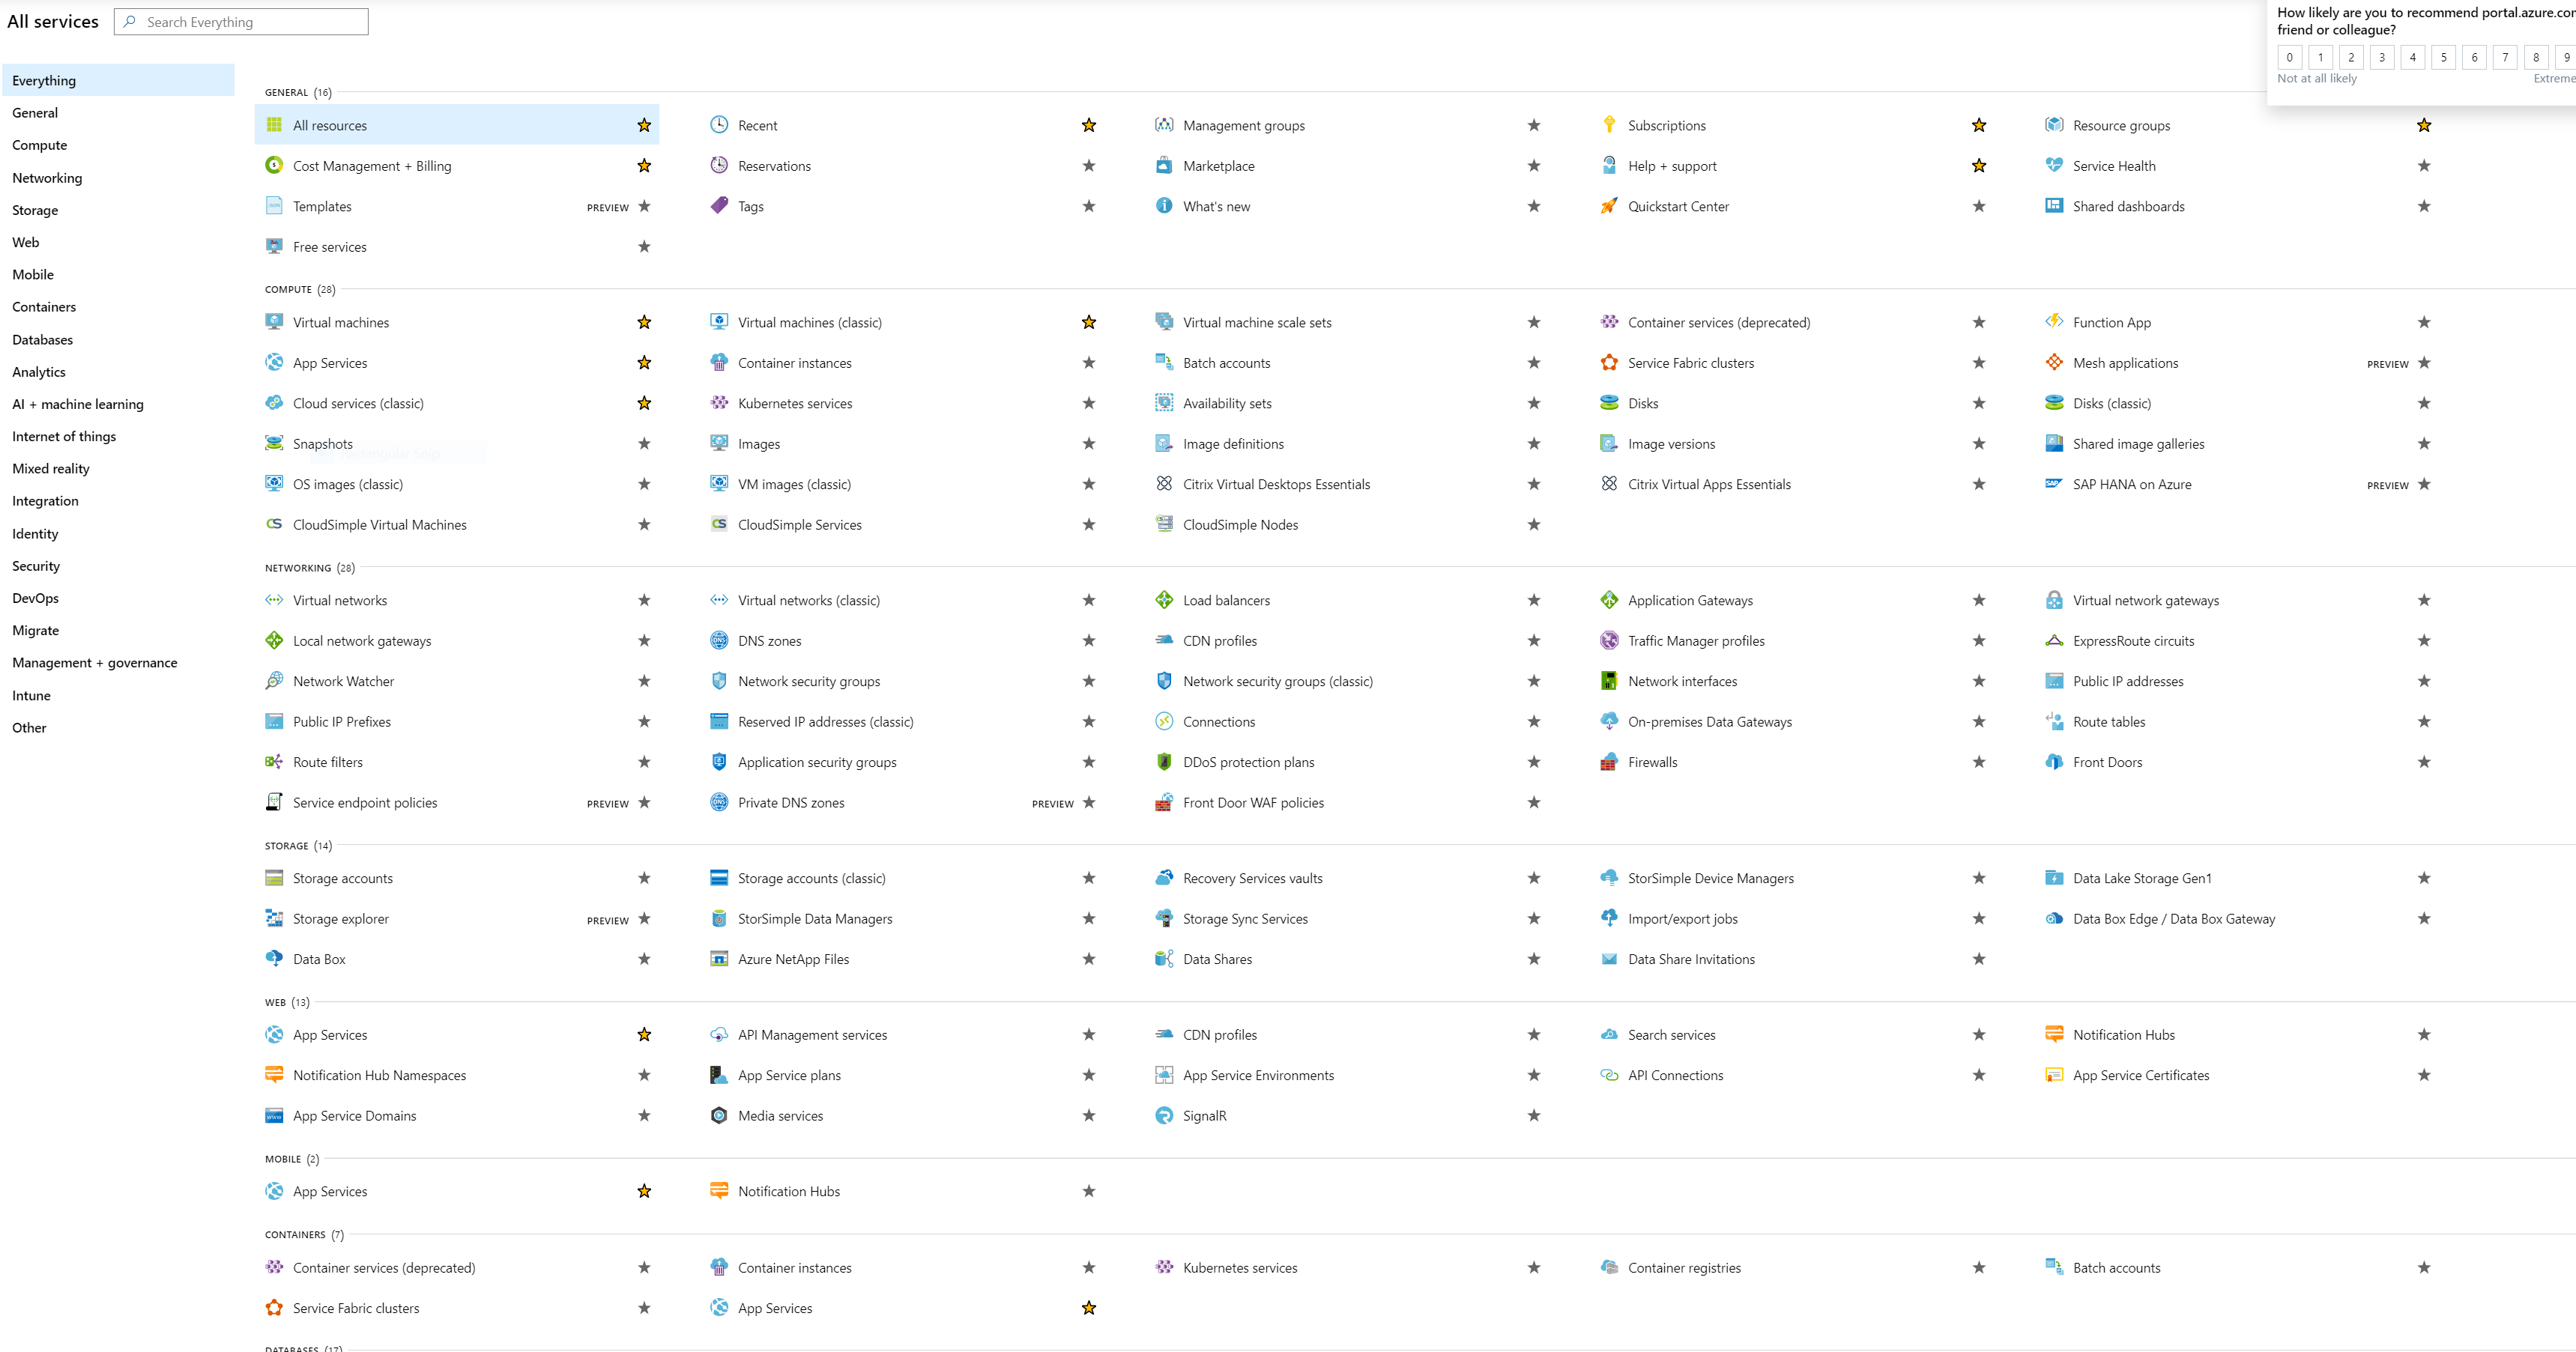
\includegraphics[width=0.95\textwidth]{azure-onderdelen.png}
    \caption{}
\end{figure}

\subsection{Samenvatting}
\begin{itemize}
    \item Wat is Cloud computing?
    \item Wie zijn de grote spelers?
    \item Welke soorten zijn er en wat zijn hun eigenschappen?
    \item Wat is een Azure subscription?
    \item Wat zijn resource groups?
    \item Hoe kan je scalen?
    \item Voor en nadelen van Azure VM’s?
    \item Wanneer Azure VM gebruiken?
    \item Wat is SQL Azure en wat zijn DTU’s?
    \item Wat is throttling?
    \item Wat is een Azure Web App?
\end{itemize}

\section{Back-end services met Azure functions}

\subsection{The Internet of \dots}

\subsubsection{The Internet of Information}
\begin{itemize}
    \item Het draait om webpagina’s met content
    \begin{itemize}
        \item Opzoeken van informatie
        \item Raadplegen van informatie
        \item E-commerce
        \item Social networks
    \end{itemize}
    \item Technologie
    \begin{itemize}
        \item HTML
        \item CSS
        \item JavaScript
        \item PHP/ASP/JAVA
    \end{itemize}
    \item Voorbeelden
    \begin{itemize}
        \item Google
        \item Facebook
        \item Amazon
        \item Stackoverflow
        \item Nieuwssites
    \end{itemize}
\end{itemize}


\subsubsection{The Internet of Services}
\begin{itemize}
    \item Connectiviteit
    \begin{itemize}
        \item Driving factor mobile applications
        \item Cross platform
        \item Data op makkelijke manier uitwissen
        \item Functionaliteit makkelijk aanroepen
        \item Centraal staan Cloud platforms
        \item REST Based
    \end{itemize}
    \item Voorbeelden
    \begin{itemize}
        \item Netflix
        \item Azure
        \item Amazon Web Services (AWS)
        \item IBM Bluemix
    \end{itemize}
\end{itemize}


\subsubsection{The Internet of Things}
= Connecting hardware

\begin{itemize}
    \item Device koppelen aan het internet
    \begin{itemize}
        \item Versturen van informatie naar cloud
        \item Toestellen praten onderling met elkaar (M2M = machine to machine)
    \end{itemize}
    \item Communicatie van/naar toestel
    \begin{itemize}
        \item We kunnen berichten sturen naar toestel
        \item We ontvangen berichten van toestel in de cloud
    \end{itemize}
    \item Voorbeelden
    \begin{itemize}
        \item Smart thermostat
        \item Smart fridge
        \item Auto's die verbonden zijn met de cloud (Tesla)
        \item Andere smart home devices (Alexa, \dots)
    \end{itemize}
\end{itemize}

Internet of Things \& Internet of services overlappen

\subsubsection{Volgende stap: The Internet of Value}

"Value" verhandelen via het internet

\begin{itemize}
    \item Bitcoin
    \item Andere cryptocurrencies
\end{itemize}

Onderliggende technologie veel belangrijker: Blockchain

\begin{itemize}
    \item Distributed ledger (grootboek)
    \item Registreren van transacties in die ledger
    \item Iedere transactie bevat een verwijzing naar de vorige transacties (chain, linked list)
\end{itemize}

\bold{Blockchain}
\begin{itemize}
    \item Public
    \item Gratis
    \item Open
\end{itemize}

\begin{itemize}
    \item Private blockchain mogelijk
    \begin{itemize}
        \item Veel evolutie in de wereld van de fintech
        \item Etherium
        \item Smart contracts
    \end{itemize}
    \item IoT \& blockchain zeer veel potentieel
    \item Bachelor-proef (project 4)
\end{itemize}

\begin{figure}[H]
    \centering
    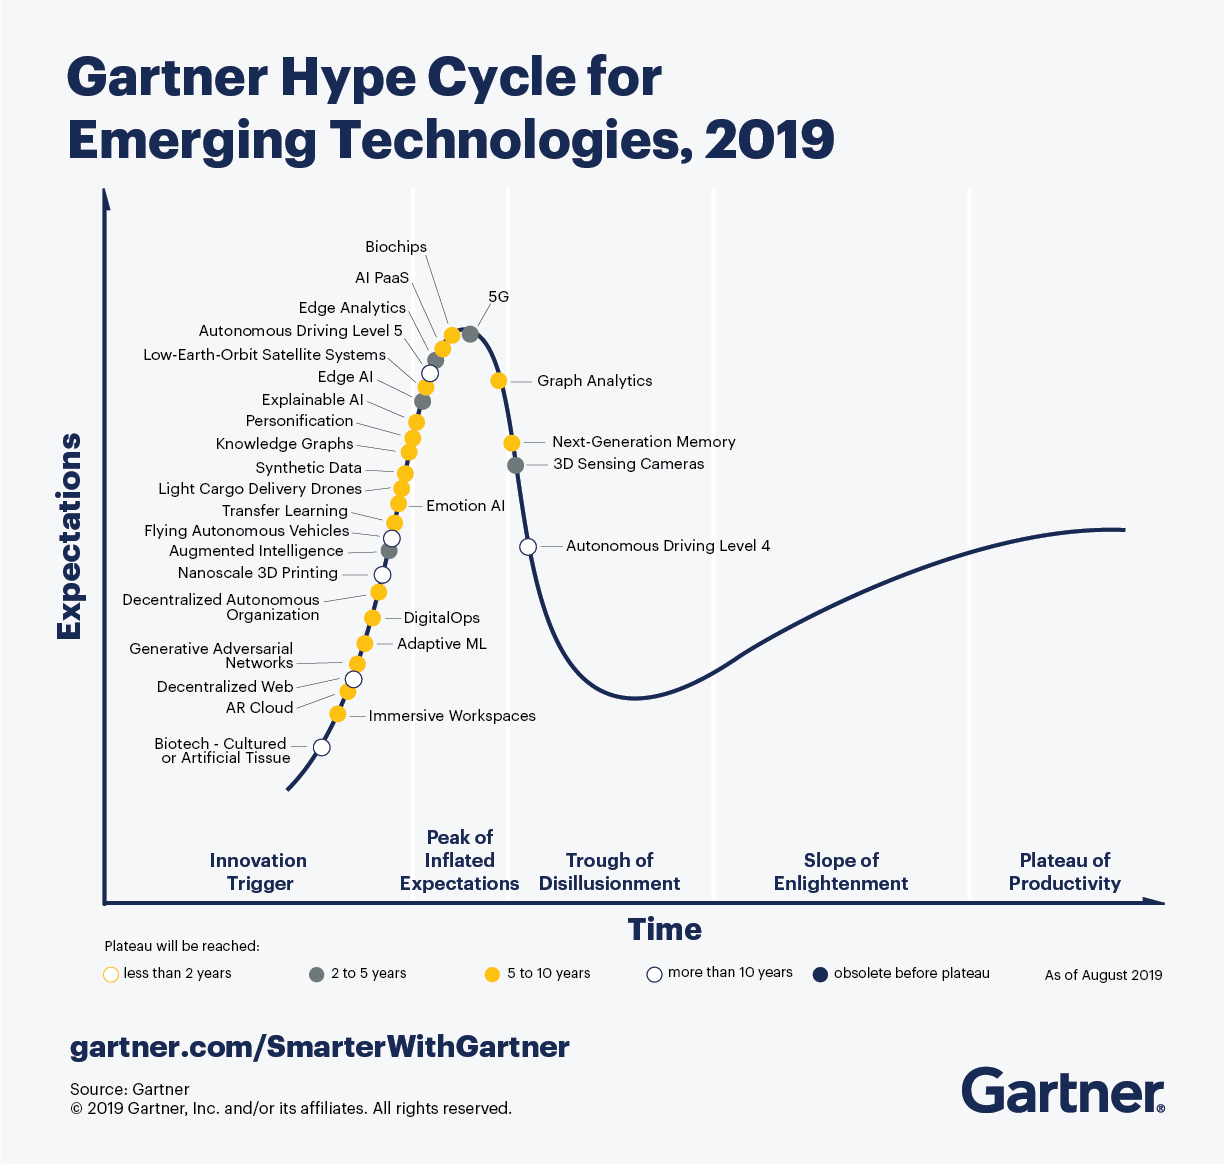
\includegraphics[width=0.6\textwidth]{gartner-hype-cycle.png}
    \caption{}
\end{figure}

Onze focus: Internet of Things \& Internet of Services

\subsection{Herhaling: Hoe werkt HTTP?}
\begin{figure}[H]
    \centering
    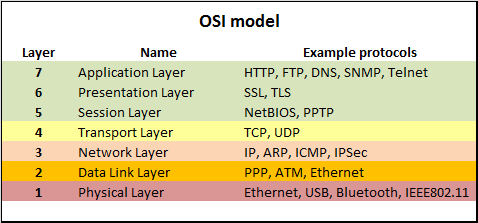
\includegraphics[width=0.5\textwidth]{osi.png}
    \caption{HTTP staat op OSI laag 7: de application layer}
\end{figure}

\begin{figure}[H]
    \centering
    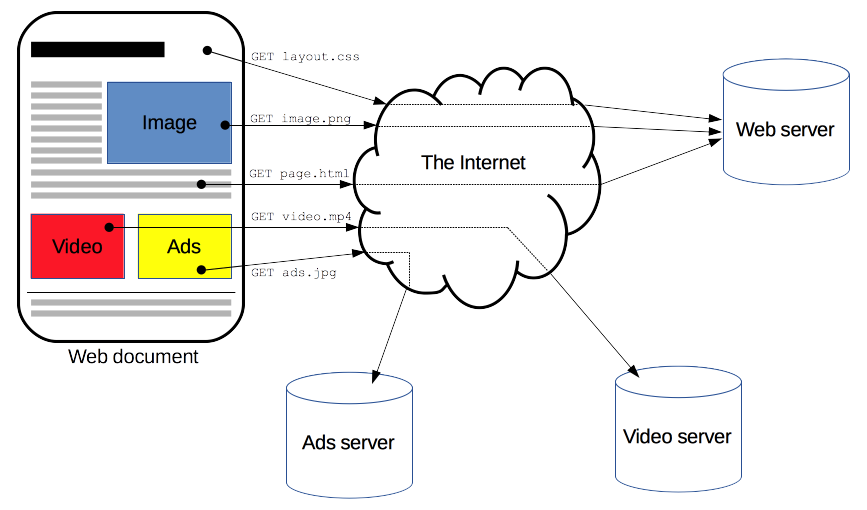
\includegraphics[width=0.5\textwidth]{http-website.png}
    \caption{Hoe werkt een website?}
\end{figure}


\subsubsection{Wat is HTTP?}
\begin{itemize}
    \item Hyper Tekst Transfer Protocol
    \item Onderliggende protocol waarop Internet werkt
    \item Opvragen van tekst, bestanden vanaf servers
    \item Request \textit{meestal} afkomstig van een webbrowser maar ook smartphone, IoT device
    \item HTTP zal bepalen hoe een request en response er moeten uitzien
    \item HTTP bevat een aantal commando’s: \bold{HTTP Verbs}
    \item HTTP is \bold{stateless}, het zal dus geen rekening houden met voorgaan requests ("Fire and Forget")
    \item HTTP is \bold{niet sessionless}, we kunnen cookies (client-side) gebruiken om data bij te houden
    \item HTTP is relatief eenvoudig: volledig text-based
\end{itemize}

\subsubsection{HTTP Verbs}
= HTTP commands/methods

\begin{itemize}
    \item \bold{GET} - ophalen data (safe: wijzigt niets op server) (SELECT)
    \item \bold{POST} - Toevoegen data: vb: formulier (INSERT)
    \item \bold{PUT} - Idempotent => meerdere requests => zelfde effect (UPDATE)
    \item \bold{DELETE} - Idempotent => meerdere requests => zelfde effect (DELETE)
\end{itemize}

\subsubsection{HTTP status code}
HTTP Response bevat naast data (html of andere) ook een status code: 

\begin{itemize}
    \item 1xx: informatief
    \item 2xx: success
    \item 3xx: redirection
    \item 4xx: client error
    \item 5xx: server error
\end{itemize}

Niet altijd evident om te weten wat je moet kiezen !

\subsubsection{HTTPS}

\begin{itemize}
    \item Beveiligen van transport
    \item Geen beveiliging van de data
    \item Defacto standaard, zonder HTTPS mag je eigenlijk \bold{niet} in productie plaatsen
    \item Browsers melden dit reeds, vb:Chrome
\end{itemize}

\begin{figure}[H]
    \centering
    
\includegraphics[width=0.3\textwidth]{https.png}
    \caption{HTTPS info in Google Chrome. Hier: geen HTTPS verbinding, enkel HTTP}
\end{figure}

\subsubsection{HTTP Request}
\begin{figure}[H]
    \centering
    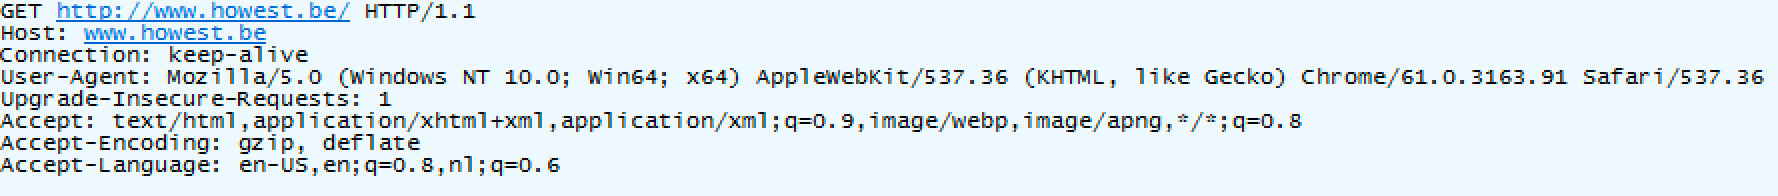
\includegraphics[width=0.8\textwidth]{http-request.png}
    \caption{HTTP GET-Request}
\end{figure}

\begin{itemize}
    \item Belangrijkste HTTP Header info: User-Agent zal dit opstellen
    \item GET = HTTP verb
    \item Host = de server
    \item User-Agent = browser info
    \item Accept = welke type data kan de client ontvangen
\end{itemize}

\subsubsection{HTTP Response}
\begin{figure}[H]
    \centering
    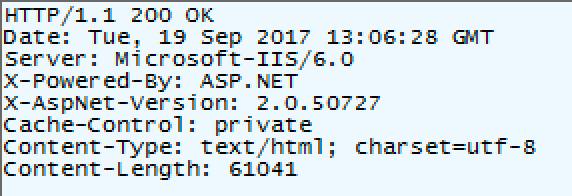
\includegraphics[width=0.5\textwidth]{http-response.png}
    \caption{HTTP Response met status code 200}
\end{figure}

\begin{itemize}
    \item Belangrijkste HTTP Header info: Server zal dit opstellen
    \item 200 OK = status code
    \item Content-Type = wat is het type van de info die ik ontvang, vb text/html
    \item Inhoud resource: vb: HTML code
\end{itemize}

\subsubsection{HTTP/2}

\begin{itemize}
    \item Sinds 2015 actief
    \item High-Level compatibility met HTTP/1.1 - methods, status codes, URI's en Header fields zijn hetzelfde
    \item Request multiplexing over een enkele TCP verbinding
    \begin{itemize}
        \item Meerdere request in parallel mogelijk over 1 tcp connection
        \item Asychroon downloaden van meerdere bestanden mogelijk
    \end{itemize}
    \item Header compression (optimalisatie van het netwerk)
    \item Binary Protocol (HTTP/1.1 is tekst protocol)
    \item HTTP/2 Server push: staat een HTTP/2-server toe om resources te sturen naar een HTTP/2-compatibele client voor de client ze vraagt (=performancetechniek)
\end{itemize}


\subsection{Webservices}
= functies die we kunnen aanroepen via het internet

\begin{itemize}
    \item Opvragen van data via het internet
    \item Devices aanspreekbaar maken via het internet
    \item Protocol is default (HTTP)
    \item Technologie-onafhankelijk (Java, C\#, PHP, Python)
    \item Platform-onafhankelijk (Windows, Linux, Android, iOS)
    \item 2 Protocollen:
    \begin{itemize}
        \item SOAP (verouderd, meestal gebruikt tss 2000-2010, gebruiken wij niet)
        \item REST (onze keuze)
    \end{itemize}
    \item Datatransport (formaat van de data) via
    \begin{itemize}
        \item XML
        \item JSON
    \end{itemize}
\end{itemize}

\subsubsection{Open data}
= data die vrij beschikbaar is

\begin{itemize}
    \item Opvraagbaar via webservices
    \item Meer en meer steden stellen data beschikbaar:
    \begin{itemize}
        \item Gent: \url{https://data.stad.gent/}
        \item Federale overheid: \url{http://data.gov.be/en}
    \end{itemize}
\end{itemize}

\subsubsection{Cognitive services}
\begin{itemize}
    \item = AI API op Azure
    \begin{itemize}
        \item \url{https://azure.microsoft.com/en-us/services/cognitive-services/}
        \item Spraak
        \item Beeldherkenning
        \item Taal
        \item \dots
    \end{itemize}
\end{itemize}

\subsubsection{Internet of Things}
\begin{itemize}
    \item Philips Hue API (\url{http://developers.meethue.com/)})
    \item Parrot AR Drone (\url{https://github.com/andrew/ar-drone-rest})
\end{itemize}

Alle voorgaande voorbeelden:
\begin{enumerate}
    \item Maken gebruik van HTTP
    \item GET/POST request naar device
    \item In de body van het request: JSON data
    \item Cross-platform
\end{enumerate}

Deze manier van werken zal je ongeveer altijd tegenkomen!

\subsubsection{JSON}

\begin{itemize}
    \item Het meest gebruikte formaat voor data is XML en JSON (wij kiezen voor JSON)
    \item De data die je terugkrijgt zal altijd mappen met een object aan de serverkant
\end{itemize}

\bold{JSON = JavaScript Object Notation}

\begin{itemize}
    \item Eenvoudig, zeer licht formaat
    \item We schrijven alles tussen accolades
    \item Basis is altijd key:value pair
    \begin{itemize}
        \item De key = lowercase, altijd tussen quotes
        \item Value: indien string $\Rightarrow$ quotes
        \item Key en value geschieden door een dubbelpunt :
        \item Key:value koppels geschieden door een komma ,
    \end{itemize}
    \begin{itemize}
        \item Validatie en testen kan op \url{https://jsonlint.com/}
    \end{itemize}
\end{itemize}

\bold{Complexe JSON}

\begin{itemize}
    \item Een key kan als value terug een JSON string bevatten
    \item Daarbinnen kan je terug een key plaatsen met een nieuwe JSON string
    \item Je kan zoveel nesten als je wil.
\end{itemize}

\bold{Complexe JSON Arrays}

\begin{itemize}
    \item Wanneer er meerdere JSON objecten zijn spreken we van een array
    \item Deze plaatsen we tussen []
    \item Een key kan terug als value een array van andere JSON objecten zijn
\end{itemize}

\subsubsection{URL}
\begin{itemize}
    \item Alles is uniek identificeerbaar via een URL $\Rightarrow$ Uniform Resource Locator
    \item Gebruik \bold{geen} spaties in de URL
    \item Gebruik \bold{geen} hoofdletters
    \item Gebruik meervoud voor resource namen
    \item Gebruik GEEN HTTP Verb om operatie aan te duiden (vb: geen get of post in url)!!
\end{itemize}

Voorbeelden 

\begin{itemize}
    \item \url{http://localhost:8080/UserManagement/rest/UserService/getUser/1} 
    \begin{itemize}
        \item NIET OK: operatienaam in URL en hoofdletters
    \end{itemize}
    \item \url{http://localhost:8080/usermanagement/rest/userservice/users/1} 
    \begin{itemize}
        \item OK: resourcenaam = meervoud, gevolgd door ID van de user die we willen opvragen
    \end{itemize}
\end{itemize}

\subsubsection{Fouten}
Wat als er iets foutloopt in een service?

\begin{itemize}
    \item Wat moet ik terugkeren ?
    \item Stuur NOOIT maar dan ook NOOIT Exceptions of intern foutmeldingen van het systeem terug naar de client in productie systemen
    \item Keer een status code Internal Sever Error 500 terug met eventueel wat informatie die jij opstelt
    \item Denk na welke info je bij de foutmelding wil terugsturen
    \begin{itemize}
        \item Geen connectie informatie
        \item Geen database namen
        \item Geen SQL statements
        \item Wees voorzichtig\dots
    \end{itemize}
\end{itemize}

\subsubsection{Samenvatting}
\begin{itemize}
    \item HTTP GET
    \begin{itemize}
        \item Alleen lezen (SELECT in database)
    \end{itemize}
    \item PUT \& DELETE
    \begin{itemize}
        \item DELETE = DELETE in SQL
        \item PUT = UPDATA in database
        \item Idempotent methodes $\Rightarrow$ voer je ze 1x uit of 100x, het resultaat blijft hetzelfde
    \end{itemize}
    \item HTTP POST
    \begin{itemize}
        \item INSERT in SQL
    \end{itemize}
\end{itemize}

\bold{Webservices zijn stateless}

\begin{itemize}
    \item Geen state van de client bijhouden aan serverkant
    \item Geen sessies gebruiken
    \item Bij iedere request naar de server moet ja alle info meesturen zodat server het request kan afhandelen
    \item Ieder request is onafhankelijk van elkaar
    \item Dit verhoogt de schaalbaarheid
    \item Eenvoudiger applicatie design
    \item Vb: vanuit een mobile app vragen we sensor data op via webservice. 
    De gebruiker van de app kan een filter instellen en wil enkel de temperatuur sensor data zien. 
    Dit wil zeggen bij iedere request naar de server MOET je meegeven welke data de gebruiker wil zien. 
    Je mag aan de server kant NIET bijhouden welke gebruiker welke sensors data wenst te zien
\end{itemize}

\subsubsection{Hoe maken we webservices?}

\begin{itemize}
    \item Aanwezig op ieder platform
    \item PHP
    \begin{itemize}
        \item Laraval, Lumen, Wave
    \end{itemize}
    \item Python
    \begin{itemize}
        \item Eve, Flask-Restfull
    \end{itemize}
    \item .NET
    \begin{itemize}
        \item ASP.NET Core met C\#
        \item Azure Functions
        \begin{itemize}
            \item Met C\#, NodeJS of Python
        \end{itemize}
    \end{itemize}
\end{itemize}

\subsection{Azure Functions}
= Serverless functions 

\subsubsection{Waarom?}
\begin{itemize}
    \item Eenvoudig concept, zeer eenvoudig aan te maken
    \item Ondersteuning voor verschillende talen
    \begin{itemize}
        \item Wij gebruiken C\# maar Python kan ook: \url{https://docs.microsoft.com/en-us/azure/azure-functions/functions-reference-python}
    \end{itemize}
    \item Snel en eenvoudig schaalbaar
    \item Geen zorgen over servers en serverbeheer (serverless)
\end{itemize}

\subsection{Azure Functions security}
\begin{itemize}
    \item Iedereen kan functies aanspreken
    \item Geen controle over wie wat doet
    \item Een hacker kan de factuur doen oplopen door constant de service aan te roepen
    \item Andere normale gebruikers zullen tragere API aanroepen krijgen
    \item Concreet: we moeten dit proberen te vermijden
\end{itemize}

3 soorten security

\begin{enumerate}
    \item Anonymous
    \begin{itemize}
        \item Iedereen kan de functie aanroepen
    \end{itemize}
    \item Function
    \begin{itemize}
        \item Er zal een function key meegegeven worden via de URL
        \item Deze key kan alleen gebruikt worden bij de gekozen functie
    \end{itemize}
    \item Admin 
    \begin{itemize}
        \item De admin key zal mee moeten verstuurd worden via de URL
        \item Deze key kan gebruikt worden voor alle functies binnen de applicatie
    \end{itemize}
\end{enumerate}

In code: via HttpTrigger

\begin{figure}[H]
    \centering
    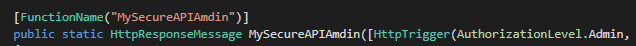
\includegraphics[width=0.7\textwidth]{azure-security-1.png}
    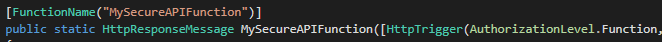
\includegraphics[width=0.7\textwidth]{azure-security-2.png}
    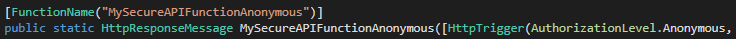
\includegraphics[width=0.7\textwidth]{azure-security-3.png}
    \caption{}
\end{figure}

\begin{figure}[H]
    \centering
    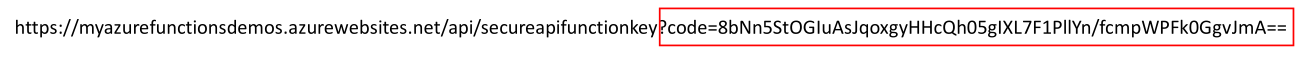
\includegraphics[width=0.7\textwidth]{azure-security-4.png}
    \caption{De key zit in de URL}
\end{figure}

\subsubsection{Voordelen van key security}
\begin{itemize}
    \item Makkelijk op te zetten
    \item Beheer keys valt mee bij niet veel gebruikers
    \item Ideaal voor scenario waar je control hebt over de client
    \begin{itemize}
        \item Vb: je interne Android of iOS hebt (app niet publiek in store)
        \item Vb: interne web applications
    \end{itemize}
\end{itemize}

\subsubsection{Nadelen van key security}
\begin{itemize}
    \item Key moet in de applicatie zitten die we verspreiden
    \begin{itemize}
        \item Vb publieke mobile app’s die iedereen kan downloaden
    \end{itemize}
    \item Bij zeer veel gebruikers zal key management lastig worden
\end{itemize}

\bold{Oplossing:}

\begin{itemize}
    \item JWT tokens
    \item Inloggen via:
    \begin{itemize}
        \item Facebook
        \item Twitter
        \item Google Account
        \item Microsoft Account
    \end{itemize}
\end{itemize}

\subsection{Andere Azure Functions}
\begin{itemize}
    \item HTTPTrigger
    \begin{itemize}
        \item Webservice
    \end{itemize}
    \item Timer trigger
    \begin{itemize}
        \item via cron expressie de functie op een tijdstip uitvoeren
        \item 0 * /5 * * * *  (=once every five minutes)
        \item \url{https://docs.microsoft.com/en-us/azure/azure-functions/functions-bindings-timer}
    \end{itemize}
    \item IoT Hub Trigger
    \item \dots
\end{itemize}

\subsection{What's next}
Welke nieuwe technologie moeten we volgen?

\begin{itemize}
    \item GraphQL (\url{https://graphql.org/})
    \begin{itemize}
        \item Query taal voor API
        \item We sturen queries door naar de API die resultaten zal terugkeren
        \item In volle ontwikkeling
    \end{itemize}
    \item gRPC (\url{https://grpc.io/})
    \begin{itemize}
        \item Open Source Remote Procedure Framework
        \item We roepen methodes aan op remote servers
        \item Platform onafhankelijk en open source
        \item Enkel HTTP/2
    \end{itemize}
    \item Mooie onderzoeksvragen voor Project 4 in 3MCT
\end{itemize}

\subsection{Azure met Raspberry Pi}
\subsubsection{4 scenario's}

\begin{enumerate}
    \item HTTP GET ophalen van data uit Webservice op Azure
    \item HTTP POST naar Webservice op Azure
    \item HTTP PUT updaten van data
    \item HTTP DELETE verwijderen van data
\end{enumerate}

\begin{itemize}
    \item Wij maken gebruik van Python op de Raspberry Pi of op de PC
    \item Andere mogelijkheden zijn JavaScript, C\#, C++, \dots
    \item Standaard geen support voor HTTP Requests
    \begin{itemize}
        \item Wij maken gebruik van Python Requests library
        \item Zeer eenvoudig in gebruik
        \item Goede documentatie: \url{http://docs.python-requests.org/en/v0.10.6/}
        \item Gebruik User Guide uit de documentatie
    \end{itemize}
\end{itemize}

\subsubsection{GET}

\begin{figure}[H]
    \centering
    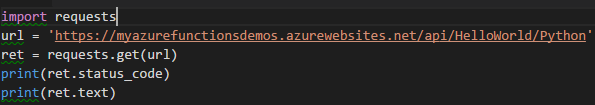
\includegraphics[width=0.6\textwidth]{rpi-request.png}
    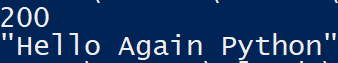
\includegraphics[width=0.3\textwidth]{rpi-response.png}
    \caption{HTTP GET request en response}
\end{figure}

Werking: 
\begin{itemize}
    \item Importeren requests library
    \item url opstellen die we willen aanroepen
    \item Get() methode uitvoeren met url
    \item status\_code = HTTP Statuscode
    \item text = inhoud van response
\end{itemize}

\subsubsection{POST}

\begin{figure}[H]
    \centering
    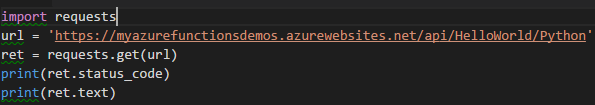
\includegraphics[width=0.6\textwidth]{rpi-request.png}
    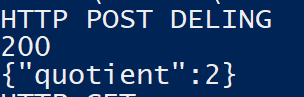
\includegraphics[width=0.3\textwidth]{rpi-response2.png}
    \caption{HTTP POST request en response}
\end{figure}

\begin{itemize}
    \item Importeren van requests + json
    \item Payload bevat Python dictionary
    \item Deze omzetten naar json string via json.dumps
    \item Via request.post kunnen we de data parameter opvullen met json in de body
    \item We krijgen statuscode terug
    \item We krijgen inhoud van body terug
\end{itemize}

\begin{figure}[H]
    \centering
    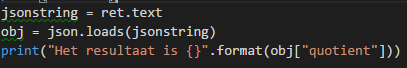
\includegraphics[width=0.6\textwidth]{rpi-response2-2.png}
    \caption{Hoe kunnen we de ontvangen JSON inladen en opvragen?}
\end{figure}

\begin{itemize}
    \item Ontvangen JSON string opslaan in variabele
    \item Ontvangen JSON string inladen via load in een dictionary
    \item Daarna kunnen we de waarden uit de dictionary opvragen zoals normaal
\end{itemize}

\subsection{Azure via .NET}
\begin{itemize}
    \item HttpClient gebruiken in .NET
    \item Zie les device programming
\end{itemize}


\subsection{Samenvatting}
\begin{itemize}
    \item Over welke soorten "Internet" spreken we ?
    \item Wat zijn Webservices en hun eigenschappen
    \item Wanneer moet je GET POST PUT DELETE gebruiken
    \item Welk HTTP verbs zijn idempotent
    \item Welke statuscodes moet ik terugsturen
    \item Wat is JSON en zorg dat je manueel JSON kan schrijven
    \item Hoe kan je Azure Functions aanroepen vanuit Python
    \item Welk soorten Azure Functions zijn er
    \item Wat is een cron expression
\end{itemize}


\section{Examen}
\begin{itemize}
    \item Theorie: 30\%
    \item Labo 70\%
    \item Het examen bevat zeker vragen over ofwel MQTT ofwel IoT
\end{itemize}

\end{document}